\section{Einleitung}
Der zunehmende Anteil der älteren Menschen in Staaten mit hoch entwickelter Industrie, wozu auch unter anderem Deutschland gehört, stellt in dem Sinne ein Problem dar, als dass eine Betreuung, falls benötigt, in den eigenen vier Wänden sich als sehr aufwändig gestaltet. Pflegeunternehmen kosten viel Geld und die eigene Familie ist nicht immer in der Lage, rund um die Uhr für die betroffene Person da zu sein. Da jedoch das Unabhängigkeitsgefühl und das gewohnte Zuhause eine große Rolle spielen, müssen andere Wege gefunden werden, um den Menschen ein altersgerechtes Wohnen bis in die späten Lebensjahre zu ermöglichen.
\\
\\
Hierfür gibt es bereits seit 2008 diverse Studien, die sich mit der Unterstützung durch technische Hilfsmittel beschäftigen. Das sogenannte \glqq Ambient-Assisted-Living\grqq \cite{aal} konzentriert sich dabei auf die Vernetzung des Wohnraumes an sich und mit externen Dienstleistern, um einerseits das alltägliche Leben durch spezielle Haushaltsgeräte oder Sicherheitssysteme zu unterstützen. Andererseits kann durch die Überwachung der vitalen Lebensfunktionen durch einen externen Dienstleister garantiert werden, dass im Notfall schnell Hilfe vor Ort ist \cite{aaltm}. Diese Überwachung kann beispielsweise durch am oder im Körper platzierte Sensoren, die die Vitalwerte messen und an eine Basisstation schicken, umgesetzt werden. Gleichzeitig werden diese Daten an eine zentrale Stelle, beispielsweise das Krankenhaus oder ein externer Dienstleister, gesendet, gespeichert so wie ausgewertet. Im Idealfall schränken solche Systeme den Nutzer in seinen alltäglichen Handlungen nicht ein und integrieren sich problemlos in sein Umfeld.

\begin{figure}[h]
\begin{center}
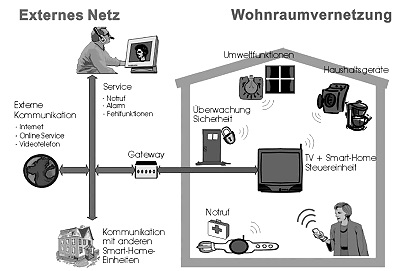
\includegraphics[scale=0.9]{images/intelligente-vernetzung.jpg} 
\caption{Schematische Darstellung eines AAL-Systems}
\end{center}
\end{figure}

\subsection{Problemstellung}
In dem Projekt, was die folgende Arbeit näher beschreibt, sollte ein solches AAL-System zur Überwachung der vitalen Lebensfunktionen als eine XML-Anwendung umgesetzt werden. Dabei wird angenommen, dass es Sensoren gibt, die in regelmäßigen Abständen Vitalwerte an eine zentrale Einheit schicken. Diese Werte umfassen die Körpertemperatur, den Herzschlag, die Atemfrequenz sowie den Blutdruck. Die Werte werden in einer zentralen Datenbank abgespeichert, um zu jederzeit verschiedene Analysen über die gesammelten Werte erstellen zu können. Außerdem werden die Daten an eine Webapplikation geschickt, mit dieser sich alle Werte für eine bestimmte Person überwachen lassen. Sollte ein Wert eine kritische Grenze überschreiten, wird dem Nutzer eine Meldung ausgegeben, worauf dieser entsprechende Maßnahmen einleiten kann.

\subsection{Aufgabenverteilung}